% Options for packages loaded elsewhere
\PassOptionsToPackage{unicode}{hyperref}
\PassOptionsToPackage{hyphens}{url}
\PassOptionsToPackage{dvipsnames,svgnames,x11names}{xcolor}
\documentclass[
  11pt,
]{article}
\usepackage{xcolor}
\usepackage[margin=1.1in]{geometry}
\usepackage{amsmath,amssymb}
\setcounter{secnumdepth}{-\maxdimen} % remove section numbering
\usepackage{iftex}
\ifPDFTeX
  \usepackage[T1]{fontenc}
  \usepackage[utf8]{inputenc}
  \usepackage{textcomp} % provide euro and other symbols
\else % if luatex or xetex
  \usepackage{unicode-math} % this also loads fontspec
  \defaultfontfeatures{Scale=MatchLowercase}
  \defaultfontfeatures[\rmfamily]{Ligatures=TeX,Scale=1}
\fi
\usepackage{lmodern}
\ifPDFTeX\else
  % xetex/luatex font selection
\fi
% Use upquote if available, for straight quotes in verbatim environments
\IfFileExists{upquote.sty}{\usepackage{upquote}}{}
\IfFileExists{microtype.sty}{% use microtype if available
  \usepackage[]{microtype}
  \UseMicrotypeSet[protrusion]{basicmath} % disable protrusion for tt fonts
}{}
\makeatletter
\@ifundefined{KOMAClassName}{% if non-KOMA class
  \IfFileExists{parskip.sty}{%
    \usepackage{parskip}
  }{% else
    \setlength{\parindent}{0pt}
    \setlength{\parskip}{6pt plus 2pt minus 1pt}}
}{% if KOMA class
  \KOMAoptions{parskip=half}}
\makeatother
\usepackage{longtable,booktabs,array}
\newcounter{none} % for unnumbered tables
\usepackage{calc} % for calculating minipage widths
% Correct order of tables after \paragraph or \subparagraph
\usepackage{etoolbox}
\makeatletter
\patchcmd\longtable{\par}{\if@noskipsec\mbox{}\fi\par}{}{}
\makeatother
% Allow footnotes in longtable head/foot
\IfFileExists{footnotehyper.sty}{\usepackage{footnotehyper}}{\usepackage{footnote}}
\makesavenoteenv{longtable}
\usepackage{graphicx}
\makeatletter
\newsavebox\pandoc@box
\newcommand*\pandocbounded[1]{% scales image to fit in text height/width
  \sbox\pandoc@box{#1}%
  \Gscale@div\@tempa{\textheight}{\dimexpr\ht\pandoc@box+\dp\pandoc@box\relax}%
  \Gscale@div\@tempb{\linewidth}{\wd\pandoc@box}%
  \ifdim\@tempb\p@<\@tempa\p@\let\@tempa\@tempb\fi% select the smaller of both
  \ifdim\@tempa\p@<\p@\scalebox{\@tempa}{\usebox\pandoc@box}%
  \else\usebox{\pandoc@box}%
  \fi%
}
% Set default figure placement to htbp
\def\fps@figure{htbp}
\makeatother
\setlength{\emergencystretch}{3em} % prevent overfull lines
\providecommand{\tightlist}{%
  \setlength{\itemsep}{0pt}\setlength{\parskip}{0pt}}
\usepackage{bookmark}
\IfFileExists{xurl.sty}{\usepackage{xurl}}{} % add URL line breaks if available
\urlstyle{same}
\hypersetup{
  colorlinks=true,
  linkcolor={blue},
  filecolor={Maroon},
  citecolor={Blue},
  urlcolor={Blue},
  pdfcreator={LaTeX via pandoc}}

\author{}
\date{}

\begin{document}

\section{Twin Counting Units: A Model-Free Test for Exact-Tie Anomalies
in Election Returns, with Evidence from Two Korean
Elections}\label{twin-counting-units-a-model-free-test-for-exact-tie-anomalies-in-election-returns-with-evidence-from-two-korean-elections}

Sangwon Seo · sangwon0001@gmail.com

\emph{Draft v1 --- June 10, 2026. Data \& code:
github.com/sangwon0001/election-simulator, archived at DOI
\href{https://doi.org/10.5281/zenodo.20624234}{10.5281/zenodo.20624234}
(fully reproducible).}

\begin{center}\rule{0.5\linewidth}{0.5pt}\end{center}

\subsection{Abstract}\label{abstract}

In the 2026 Korean nationwide local elections, nine ``twin'' pairs of
counting units --- distinct (neighborhood × vote-type) units whose two
leading candidates received exactly identical vote counts --- reignited
public election-fraud controversies. Using the complete official returns
(17 provinces, \textasciitilde7,000 counting units), we measure how
surprising this is. First, a multinomial--binomial generative model with
per-unit observed parameters yields an expected 3.23 twins and
P(\(\geq 9\)) = 0.64\%. Second, we prove that such plug-in
(parametric-bootstrap) procedures underestimate the collision
probability of truly identical-parameter pairs by a factor of
\(1/\sqrt{2}\) per matched dimension --- a noise double-counting bias
--- and propose as a complement a \textbf{model-free sideband
estimator}, the bump-hunt analogue for exact ties, which extrapolates
lattice-shell near-pair counts to distance zero. The sideband estimate,
3.47 ± 0.18 expected twins with P(\(\geq 9\)) = 0.94\% {[}0.49, 1.66{]},
converges with the generative model, as does an unconditional
distribution-based (ab-initio) simulation (\textasciitilde1\%). Third, a
pre-specified replication on the 2025 presidential election shows no
excess (7 observed vs.~6.02 expected, P = 39.7\%), with near-pair
density ratios and vote-type composition matching the model. Fourth,
type decomposition localizes the local-election anomaly: all five
Gwangju--Jeonnam twins fall in the early-voting pair type with the
\emph{smallest} expectation (conditional P \(\approx\) 0.2\%, post hoc),
so the anomaly is confined to ``local elections × Gwangju--Jeonnam ×
early voting × exact ties.'' We conclude that (i) twins are a baseline
natural phenomenon; (ii) the 2026 excess is a \textasciitilde1\% tail
event --- too rare for ``entirely natural,'' far too common for
``evidence of fraud''; and (iii) the residual identity of the excess
(chance vs.~a non-statistical cause) is unidentifiable from a single
election. As a by-product we show that the key assumption of the public
analysis that sparked the debate --- a 1\% ``similar-pair'' rate --- is
about 80× too large (measured: 0.012\%).

\textbf{Keywords}: election forensics, exact ties, birthday problem,
parametric bootstrap, bump hunt, post-hoc selection

\begin{center}\rule{0.5\linewidth}{0.5pt}\end{center}

\subsection{1. Introduction}\label{introduction}

\subsubsection{1.1 The controversy}\label{the-controversy}

Immediately after the 9th Korean nationwide local elections (June 3,
2026), it was noticed that in the Incheon mayoral race the two leading
candidates' early-voting counts in two neighborhoods of Songdo
(Yeonsu-gu) coincided exactly at (3,030, 1,440), and that the South
Jeolla gubernatorial race contained five such ``twin'' pairs. Fraud
allegations followed. A statistician responded with a public analysis
arguing, via a coin-flipping model and birthday-problem logic, that the
coincidences are ``mathematically natural'' {[}8{]}; rebuttals and
counter-rebuttals ensued. Both sides argued from weak quantitative
ground: the suspicious side never computed the base rate of exact ties,
while the rebuttal substituted an assumption for the load-bearing
parameter of its own argument (a ``1\% similar-pair rate'').

\subsubsection{1.2 Research question and
contributions}\label{research-question-and-contributions}

Our question is simple: \textbf{is the observed number of twins
compatible with the base rate predicted by a smooth stochastic model?}
We make four contributions.

\begin{enumerate}
\def\labelenumi{\arabic{enumi}.}
\tightlist
\item
  \textbf{Measurement.} Using the complete official returns we measure
  both the observed twin counts and their expectation --- by
  model-dependent and model-free routes --- replacing the assumptions of
  the public debate with measured quantities.
\item
  \textbf{A methodological warning.} We prove that plug-in simulations
  which redraw counts around observed parameters systematically
  underestimate exact-tie probabilities, and characterize when and by
  how much (\(1/\sqrt{2}\) per dimension; Proposition 1).
\item
  \textbf{A model-free estimator.} We propose a sideband estimator of
  the expected number of exact ties --- extrapolating lattice-shell
  counts of near pairs to distance zero --- derive its unordered-pair
  normalization (Proposition 2), and validate it by simulation
  self-consistency.
\item
  \textbf{A replication design.} We pre-specify the prediction ``if the
  excess is structural it must reappear, scaled up, in another
  election,'' and test it on the 2025 presidential election, where it is
  rejected. This partially resolves the circularity inherent in post-hoc
  analysis of a single election.
\end{enumerate}

\subsubsection{1.3 Related work}\label{related-work}

Statistical detection of electoral irregularities includes digit-based
tests {[}1, 2{]}, turnout--vote-share fingerprints {[}3{]}, and
integer-percentage / duplicate-value anomalies {[}4{]}. Our object ---
exact multivariate ties between \emph{different} units --- is kin to the
duplicate analyses of {[}4{]}, but differs in that (i) we treat
two-dimensional collisions (both leading candidates simultaneously), and
(ii) we estimate the expectation not from a model but from the data's
own near-pair density, in direct analogy with the bump hunt of
high-energy physics (interpolating the expected background in a signal
region from sidebands). On the dangers of post-hoc hypothesis selection
we follow {[}5{]}.

\subsection{2. Data}\label{data}

\subsubsection{2.1 The 2026 local elections (June 3,
2026)}\label{the-2026-local-elections-june-3-2026}

We collected the complete gubernatorial/mayoral returns for all 17
provinces from the National Election Commission's election statistics
system (info.nec.go.kr) with an automated Playwright crawler. A
\textbf{counting unit} is a neighborhood (eup/myeon/dong) × vote type
\{in-precinct early voting, election-day voting\}; absentee,
out-of-precinct early votes, and overseas votes are not broken down by
neighborhood and are excluded. The two leading candidates (A, B) are
identified per province by total votes. Gwangju and South Jeolla share
the same two leading candidates (same race) and are merged into a single
block, so that cross-province pairs count; all other provinces have
distinct candidates, so only within-province pairs are meaningful. The
final data comprise \textasciitilde3,500 neighborhoods and
\textasciitilde7,100 counting units.

A convention of the source data matters: the ``registered voters'' of an
early-voting unit equals its turnout (tautologically), and a
neighborhood's total electorate equals the sum of its early-voting and
election-day registered counts.

\subsubsection{2.2 The 2025 presidential election (June 3,
2025)}\label{the-2025-presidential-election-june-3-2025}

We use the official polling-station-level CSV from the public data
portal (169,749 rows), aggregating election-day polling stations to the
neighborhood level to match the unit definition above. The presidential
election has identical candidates nationwide, so the whole country forms
a single block: 3,554 neighborhoods \(\to\) 7,108 counting units, with
\textasciitilde{}\(2.5 \times 10^{7}\) comparable pairs. (A, B) = (Lee
Jae-myung, Kim Moon-soo).

\subsubsection{2.3 Observed twins}\label{observed-twins}

The local elections produced nine twins (Table 1): five in the
Gwangju--Jeonnam block (including one cross-province pair) and one each
in Incheon, North Gyeongsang, South Gyeongsang, and North Jeolla. The
vote-type composition is six early·early, two day·day, and one mixed
pair.

\textbf{Table 1. The nine twins of the 2026 local elections}

{\def\LTcaptype{none} % do not increment counter
\begin{longtable}[]{@{}
  >{\raggedright\arraybackslash}p{(\linewidth - 10\tabcolsep) * \real{0.1667}}
  >{\raggedright\arraybackslash}p{(\linewidth - 10\tabcolsep) * \real{0.1667}}
  >{\raggedright\arraybackslash}p{(\linewidth - 10\tabcolsep) * \real{0.1667}}
  >{\raggedright\arraybackslash}p{(\linewidth - 10\tabcolsep) * \real{0.1667}}
  >{\raggedright\arraybackslash}p{(\linewidth - 10\tabcolsep) * \real{0.1667}}
  >{\raggedright\arraybackslash}p{(\linewidth - 10\tabcolsep) * \real{0.1667}}@{}}
\toprule\noalign{}
\begin{minipage}[b]{\linewidth}\raggedright
Block
\end{minipage} & \begin{minipage}[b]{\linewidth}\raggedright
Unit 1
\end{minipage} & \begin{minipage}[b]{\linewidth}\raggedright
Unit 2
\end{minipage} & \begin{minipage}[b]{\linewidth}\raggedright
A
\end{minipage} & \begin{minipage}[b]{\linewidth}\raggedright
B
\end{minipage} & \begin{minipage}[b]{\linewidth}\raggedright
Type
\end{minipage} \\
\midrule\noalign{}
\endhead
\bottomrule\noalign{}
\endlastfoot
Incheon & Songdo 1-dong, Yeonsu & Songdo 2-dong, Yeonsu & 3,030 & 1,440
& early·early \\
Gwangju--Jeonnam & Songjeong 1-dong, Gwangsan & Geumsan-myeon, Goheung &
1,401 & 120 & early·early (cross) \\
Gwangju--Jeonnam & Bukha-myeon, Jangseong & Eomda-myeon, Hampyeong & 606
& 57 & early·early \\
Gwangju--Jeonnam & Samil-dong, Yeosu & Hauido-myeon, Sinan & 506 & 42 &
early·early \\
Gwangju--Jeonnam & Iyang-myeon, Hwasun & Byeongyeong-myeon, Gangjin &
444 & 46 & early·early \\
Gwangju--Jeonnam & Nodong-myeon, Boseong & Palgeum-myeon, Sinan & 356 &
42 & early·early \\
N. Gyeongsang & Jeomgok-myeon, Uiseong & Changsu-myeon, Yeongdeok & 456
& 109 & day·day \\
S. Gyeongsang & Yangbo-myeon, Hadong & Wicheon-myeon, Geochang & 385 &
180 & day·day \\
N. Jeolla & Ungpo-myeon, Iksan & Seongsu-myeon, Jinan & 186 & 150 &
early·day \\
\end{longtable}
}

The presidential election produced seven twins (six day·day, one mixed,
zero early·early; §5).

\subsubsection{2.4 Data integrity
verification}\label{data-integrity-verification}

For all 18 counting units composing the twins of Table 1 we performed
two checks (\texttt{src/verify\_twins.py}). (i) \textbf{Internal
arithmetic consistency}: early + election-day = total (for electorate,
ballots, A, and B separately), and A + B \(\leq\) ballots --- all units
pass. (ii) \textbf{Cross-validation across independent retrievals}: the
nine Jeonnam units were collected twice, by the automated crawler and in
a separate manual crawl session; the two retrievals agree exactly on
every unit. The data therefore faithfully reflect the published official
returns, and the observed twins are not artifacts of our collection or
transcription. Errors \emph{upstream} of official publication (counting
floor \(\to\) reporting system) cannot be excluded by re-reading the
published records; that is the domain of physical recounts (§7.2).

\subsection{3. Methods}\label{methods}

\subsubsection{3.1 The canonical generative
model}\label{the-canonical-generative-model}

For neighborhood \(i\), let \(N_i\) be its electorate, \(r^e_i\) its
early-voting rate, \(r^b_i\) its election-day rate conditional on not
voting early, and \(p^t_{A,i}, p^t_{B,i}\) the leading candidates' vote
shares by vote type \(t \in \{e, b\}\) --- all set to their observed
per-neighborhood values. One realization is generated as

\[V^e_i \sim \mathrm{Bin}(N_i, r^e_i), \quad V^b_i \sim \mathrm{Bin}(N_i - V^e_i, r^b_i),\]
\[A^t_i \sim \mathrm{Bin}(V^t_i, p^t_{A,i}), \quad B^t_i \sim \mathrm{Bin}\big(V^t_i - A^t_i,\; p^t_{B,i}/(1-p^t_{A,i})\big),\]

and we count unordered pairs of units agreeing simultaneously in
\((A, B)\). The only randomness is (i) who votes early / on election day
/ abstains (multinomial) and (ii) how ballots split (binomial); there
are no free parameters. National distributions are obtained as sums over
blocks simulated with independent seeds (R =
\(5{\times}10^{4}\)--\(2{\times}10^{5}\) per block).

Robustness variants --- fixed vs.~random turnout, sub-binomial
dispersion \(\varphi < 1\), population-draw parameters,
finite-population corrections --- do not change the results (§5.1 of the
repository's research notes). We additionally run an \textbf{ab-initio
variant} that deliberately severs all parameter correlations: only the
number of neighborhoods is kept, and every realization redraws \(N_i\)
from a fitted lognormal and all rates from fitted Beta distributions
(method-of-moments). This provides an unconditional base rate to which
the criticism ``you conditioned on the observed values'' does not apply.

\subsubsection{3.2 The plug-in bias (noise
double-counting)}\label{the-plug-in-bias-noise-double-counting}

The canonical model is a parametric bootstrap that plugs observed
parameters in as truth. For exact ties this procedure carries a
systematic bias.

\textbf{Proposition 1.} Let two units share identical true parameters,
\(X_i, X_j \sim
\mathrm{Bin}(V, p)\) independently. Re-drawing around the observations,
\(X'_k \sim
\mathrm{Bin}(V, X_k / V)\), the tie probability satisfies asymptotically

\[\frac{\mathbb{E}_{\mathrm{data}}\, P(X'_i = X'_j \mid \mathrm{data})}{P(X_i = X_j)}
\;\longrightarrow\; \frac{1}{\sqrt{2}},\]

and \(2^{-d/2}\) for simultaneous ties in \(d\) coordinates.

\emph{Proof sketch.} Under the normal approximation
\(D = X_i - X_j \approx \mathcal N(0,
2\sigma^2)\) with \(\sigma^2 = Vp(1-p)\), so
\(P(D = 0) \approx (4\pi\sigma^2)^{-1/2}\). The re-drawn difference is
centered on the observed difference \(d\): \(D' \mid d \approx
\mathcal N(d, 2\sigma^2)\), and \(d\) itself is distributed
\(\mathcal N(0, 2\sigma^2)\); marginally
\(D' \approx \mathcal N(0, 4\sigma^2)\) --- the noise is convolved in
twice. The ratio of densities at zero is
\(\sqrt{2\sigma^2 / 4\sigma^2} = 1/\sqrt 2\); coordinates multiply under
independence. \(\blacksquare\)

Numerical verification (exact binomial pmf inner products; V = 2,000, 50
identical pairs plus 100 heterogeneous units, 200 observation
replicates): ratio 0.707 for identical pairs (theory \(1/\sqrt{2}\)),
0.985 (\(\approx 1\)) for heterogeneous pairs. Conversely, when the
distribution of true parameter differences is locally flat at the noise
scale the bias vanishes --- its magnitude depends on unobservable
structure (how many truly identical pairs exist) and is therefore
uncorrectable within the model. This motivates the model-free estimator
below.

\subsubsection{3.3 The model-free sideband
estimator}\label{the-model-free-sideband-estimator}

For each pair \((i, j)\) define the Chebyshev distance
\(d_{ij} = \max(|A_i - A_j|,
|B_i - B_j|)\) and the shell counts \(n(d) = \#\{i < j : d_{ij} = d\}\).
Twins are \(n(0)\).

\textbf{Proposition 2 (unordered-pair normalization).} If the
per-lattice-site density \(c\) of ordered pair differences is locally
constant near the origin, then the \(L_\infty\) shell at distance
\(d \ge 1\) contains \(8d\) lattice sites and the unordered-pair shell
count has expectation \(\mathbb E\, n(d) = 4dc\), while the origin has
\(\mathbb E\, n(0) = c/2\). Hence with \(\rho(d) \equiv n(d)/(8d)\),
\(\mathbb E\, n(0) = \rho(0)\): \textbf{the \(d \to 0\) extrapolation of
\(\rho(d)\) is itself the expected number of twins.}

\emph{Proof sketch.} Unordered pairs identify \(\pm v\); each class with
\(v \ne 0\) absorbs two lattice sites, giving \(4d\) classes per shell,
while the origin class absorbs the two ordered self-reflections, giving
expectation \(c/2\). Synthetic uniform check: \(n(0) = 87.8\)
vs.~extrapolation 85.5 (theory 88.9). \(\blacksquare\)

We fit a linear (and, as a check, quadratic) trend to \(\rho(d)\),
\(d \in [1, 15]\), by Poisson maximum likelihood, extrapolate to
\(\rho(0)\), obtain standard errors by Poisson resampling (300
replicates), and compute tail probabilities from
\(\mathrm{Poisson}(\hat\rho(0))\). \textbf{Self-validation}: applying
the same extrapolation to the generative model's own simulated shells
recovers the model's true \(d = 0\) expectation (3.24 vs.~3.27 ± 0.01).

This estimator uses no generative assumptions --- no binomiality, no
turnout model, no dispersion parameter. Its only assumption is that the
distribution of count differences between distinct units is smooth at
the ±15-vote scale near the origin, which is precisely the null
hypothesis under test. As a companion diagnostic we examine the
observed-to-model shell ratio
\(r(d) = n_{\mathrm{obs}}(d) / n_{\mathrm{sim}}(d)\): a uniformly
elevated, flat \(r(d)\) would indicate global over-smoothing by the
model (Proposition 1's bias at work), whereas \(r(d) \approx 1\) for
\(d \ge 1\) with an isolated spike at \(r(0)\) indicates an atom at
exact equality.

\subsubsection{3.4 Replication test and type
decomposition}\label{replication-test-and-type-decomposition}

We pre-specify: \emph{if the local-election excess reflects a structural
mechanism of elections in general (model misspecification, reporting
practice, demographic clustering), then the presidential election ---
whose expectation is larger --- must show a proportionally larger
absolute excess (\(6.0 \times 2.8 \approx 17\) twins).} We also
decompose expected twins by vote-type pair \{early·early, day·day,
mixed\} and compare with the observed composition. To first order the
expected density of exact ties is independent of the noise scale and is
determined by the lattice packing density of unit means,
\(\propto 1/(\text{spread}_A
\times \text{spread}_B)\); the decomposition therefore yields model and
data predictions for \emph{where} twins should occur.

\subsection{4. Results I: the 2026 local
elections}\label{results-i-the-2026-local-elections}

\subsubsection{4.1 National base rate and
significance}\label{national-base-rate-and-significance}

\textbf{Table 2. Nationwide results (9 observed twins)}

{\def\LTcaptype{none} % do not increment counter
\begin{longtable}[]{@{}lll@{}}
\toprule\noalign{}
Estimation route & Expected twins & P(\(\geq 9\)) \\
\midrule\noalign{}
\endhead
\bottomrule\noalign{}
\endlastfoot
Canonical generative model & 3.23 & 0.64\% \\
Sideband, linear extrapolation & 3.47 ± 0.18 & 0.94\% {[}0.49,
1.66{]} \\
Sideband, quadratic & 3.64 ± 0.36 & 1.26\% {[}0.33, 3.39{]} \\
\end{longtable}
}

For the Gwangju--Jeonnam block alone (5 observed): canonical expectation
1.47 with P(\(\geq 5\)) = 1.74\%; sideband 1.67 ± 0.12 with
P(\(\geq 5\)) = 2.75\%; ab-initio (unconditional, per-province/pooled
fits) expectation 1.26/1.33 with P(\(\geq 5\)) = 0.99\%/1.26\%.
\textbf{The conditional, unconditional, and model-free routes all
converge on the 1--3\% band.}

\subsubsection{4.2 Shell diagnostics: the excess is an atom at exact
equality}\label{shell-diagnostics-the-excess-is-an-atom-at-exact-equality}

\textbf{Table 3. Nationwide near-pair shells: observed vs.~model}

{\def\LTcaptype{none} % do not increment counter
\begin{longtable}[]{@{}
  >{\raggedright\arraybackslash}p{(\linewidth - 22\tabcolsep) * \real{0.0833}}
  >{\raggedright\arraybackslash}p{(\linewidth - 22\tabcolsep) * \real{0.0833}}
  >{\raggedright\arraybackslash}p{(\linewidth - 22\tabcolsep) * \real{0.0833}}
  >{\raggedright\arraybackslash}p{(\linewidth - 22\tabcolsep) * \real{0.0833}}
  >{\raggedright\arraybackslash}p{(\linewidth - 22\tabcolsep) * \real{0.0833}}
  >{\raggedright\arraybackslash}p{(\linewidth - 22\tabcolsep) * \real{0.0833}}
  >{\raggedright\arraybackslash}p{(\linewidth - 22\tabcolsep) * \real{0.0833}}
  >{\raggedright\arraybackslash}p{(\linewidth - 22\tabcolsep) * \real{0.0833}}
  >{\raggedright\arraybackslash}p{(\linewidth - 22\tabcolsep) * \real{0.0833}}
  >{\raggedright\arraybackslash}p{(\linewidth - 22\tabcolsep) * \real{0.0833}}
  >{\raggedright\arraybackslash}p{(\linewidth - 22\tabcolsep) * \real{0.0833}}
  >{\raggedright\arraybackslash}p{(\linewidth - 22\tabcolsep) * \real{0.0833}}@{}}
\toprule\noalign{}
\begin{minipage}[b]{\linewidth}\raggedright
d
\end{minipage} & \begin{minipage}[b]{\linewidth}\raggedright
0
\end{minipage} & \begin{minipage}[b]{\linewidth}\raggedright
1
\end{minipage} & \begin{minipage}[b]{\linewidth}\raggedright
2
\end{minipage} & \begin{minipage}[b]{\linewidth}\raggedright
3
\end{minipage} & \begin{minipage}[b]{\linewidth}\raggedright
4
\end{minipage} & \begin{minipage}[b]{\linewidth}\raggedright
5
\end{minipage} & \begin{minipage}[b]{\linewidth}\raggedright
6
\end{minipage} & \begin{minipage}[b]{\linewidth}\raggedright
8
\end{minipage} & \begin{minipage}[b]{\linewidth}\raggedright
10
\end{minipage} & \begin{minipage}[b]{\linewidth}\raggedright
12
\end{minipage} & \begin{minipage}[b]{\linewidth}\raggedright
15
\end{minipage} \\
\midrule\noalign{}
\endhead
\bottomrule\noalign{}
\endlastfoot
Observed & 9 & 35 & 48 & 72 & 130 & 146 & 135 & 198 & 238 & 315 & 362 \\
Model & 3.24 & 25.8 & 51.2 & 76.5 & 102.1 & 128.5 & 153.5 & 203.6 &
252.2 & 299.6 & 368.5 \\
r(d) & \textbf{2.78} & 1.36 & 0.94 & 0.94 & 1.27 & 1.14 & 0.88 & 0.97 &
0.94 & 1.05 & 0.98 \\
\end{longtable}
}

\begin{figure}
\centering
\pandocbounded{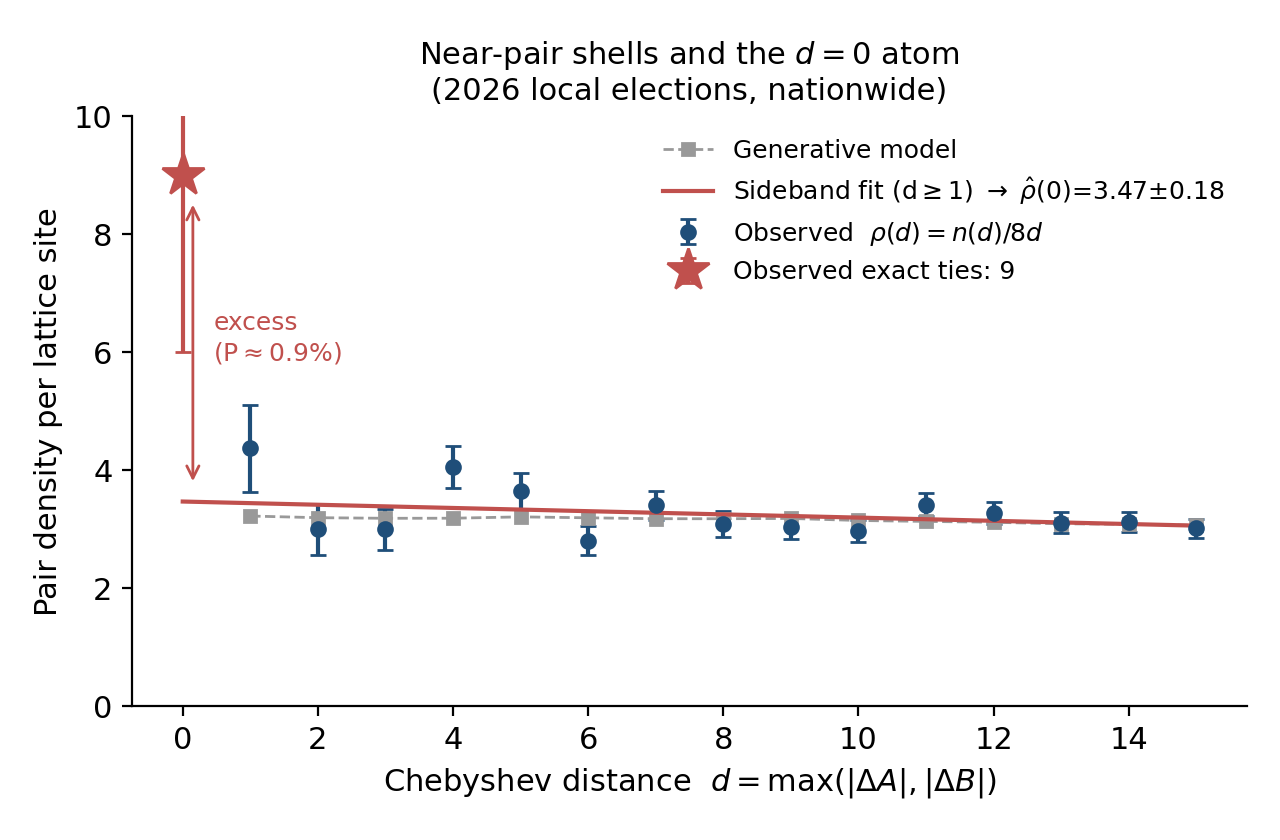
\includegraphics[keepaspectratio,alt={Figure 1}]{figs/fig1_sideband.png}}
\caption{Figure 1}
\end{figure}

\textbf{Figure 1.} Nationwide near-pair shells, 2026 local elections.
Observed density \(\rho(d)\) with Poisson error bars, generative model
(grey), and the \(d \ge 1\) sideband fit extrapolated to \(d = 0\)
(red). The gap between the nine observed exact ties (star) and the
extrapolated 3.47 is the excess under test.

For \(d \ge 2\) the ratio \(r(d)\) is flat at 0.88--1.27 (within Poisson
fluctuation): \textbf{the model reproduces the density of near-misses
exactly.} Had the hidden population of identical-parameter pairs
presupposed by Proposition 1's bias existed, \(r\) would have been
elevated across the whole range (\textasciitilde2); it is not, so the
canonical expectation 3.23 is trustworthy and its agreement with the
sideband 3.47 is independent confirmation. The only departure is at
\(d = 0\): the excess is not smooth clustering but an \textbf{atom at
exact equality}. This excludes both directions of smooth explanation at
once: a benign mechanism such as demographic similarity would also
inflate \(d = 1\)--15 (no trace), and the over-smoothing critique of the
model is refuted by \(r(d \ge 1) \approx 1\).

\subsubsection{4.3 Type decomposition: the excess sits in the
least-expected
type}\label{type-decomposition-the-excess-sits-in-the-least-expected-type}

The decomposition for the Gwangju--Jeonnam block (Table 4) reveals a
fact opposite to intuition. Election-day units are \emph{smaller} than
early-voting units (median ballots 796 vs.~1,147); both the data's own
near pairs and the model's expectation rank day·day pairs first. Yet all
five observed twins are early·early --- the type with the smallest
expectation.

\textbf{Table 4. Gwangju--Jeonnam type decomposition}

{\def\LTcaptype{none} % do not increment counter
\begin{longtable}[]{@{}llll@{}}
\toprule\noalign{}
& day·day & mixed & early·early \\
\midrule\noalign{}
\endhead
\bottomrule\noalign{}
\endlastfoot
Model expected twins & 0.58 & 0.48 & \textbf{0.42} \\
Observed near pairs (d = 1--10) & 265 & 198 & 174 \\
\textbf{Observed twins} & 0 & 0 & \textbf{5} \\
\end{longtable}
}

\begin{figure}
\centering
\pandocbounded{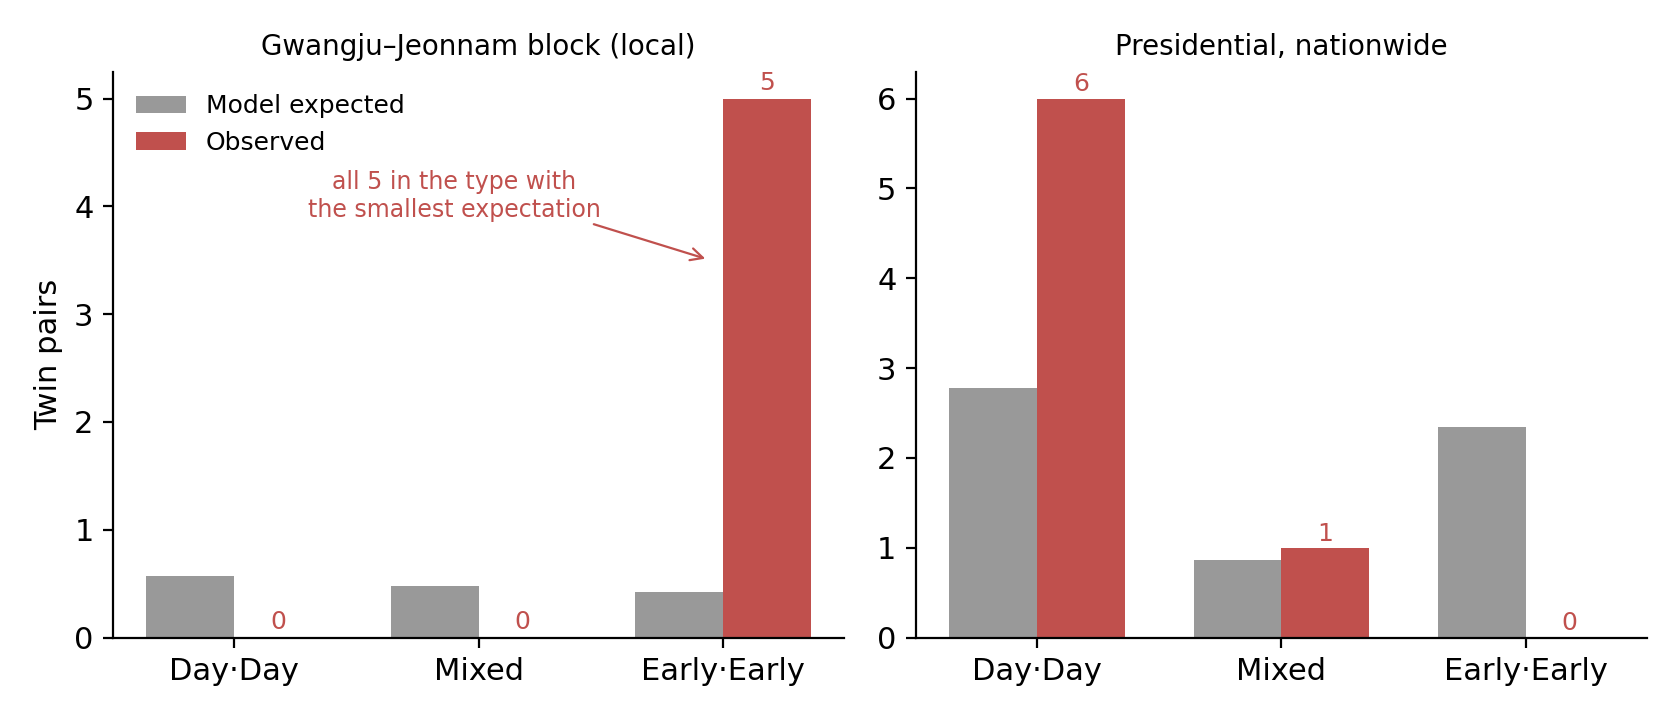
\includegraphics[keepaspectratio,alt={Figure 3}]{figs/fig3_types.png}}
\caption{Figure 3}
\end{figure}

\textbf{Figure 3.} Expected (grey) vs.~observed (red) twins by type.
Left: Gwangju--Jeonnam (local) --- all five observed twins fall in the
least-expected type. Right: presidential --- observed composition
matches expectation.

Conditioning on the total,
\(P(\text{all 5 early·early} \mid \text{type share } 28.4\%) =
0.284^5 \approx 0.19\%\) --- an anomaly \emph{additional} to the count
excess (1.7\%). It is a post-hoc statistic, selected after seeing the
data, and should be discounted for the exploration degrees of freedom
(three types, block choice); it remains hard to dismiss after that
discount. In sum the anomaly is localized four-fold: \textbf{local
elections × Gwangju--Jeonnam × early voting × exact equality}. The
popular benign account --- ``landslide × small rural units, hence
natural'' --- fails the type decomposition, since the same logic
predicts a day·day majority.

\subsection{5. Results II: replication --- the 2025 presidential
election}\label{results-ii-replication-the-2025-presidential-election}

The identical pipeline applied to the nationwide single block (7,108
units):

\textbf{Table 5. Presidential election (7 observed twins)}

{\def\LTcaptype{none} % do not increment counter
\begin{longtable}[]{@{}lll@{}}
\toprule\noalign{}
Estimation route & Expected & P(\(\geq 7\)) \\
\midrule\noalign{}
\endhead
\bottomrule\noalign{}
\endlastfoot
Canonical generative model & 6.02 & 39.7\% \\
Sideband, linear extrapolation & 6.44 ± 0.24 & 46.3\% \\
\end{longtable}
}

\begin{figure}
\centering
\pandocbounded{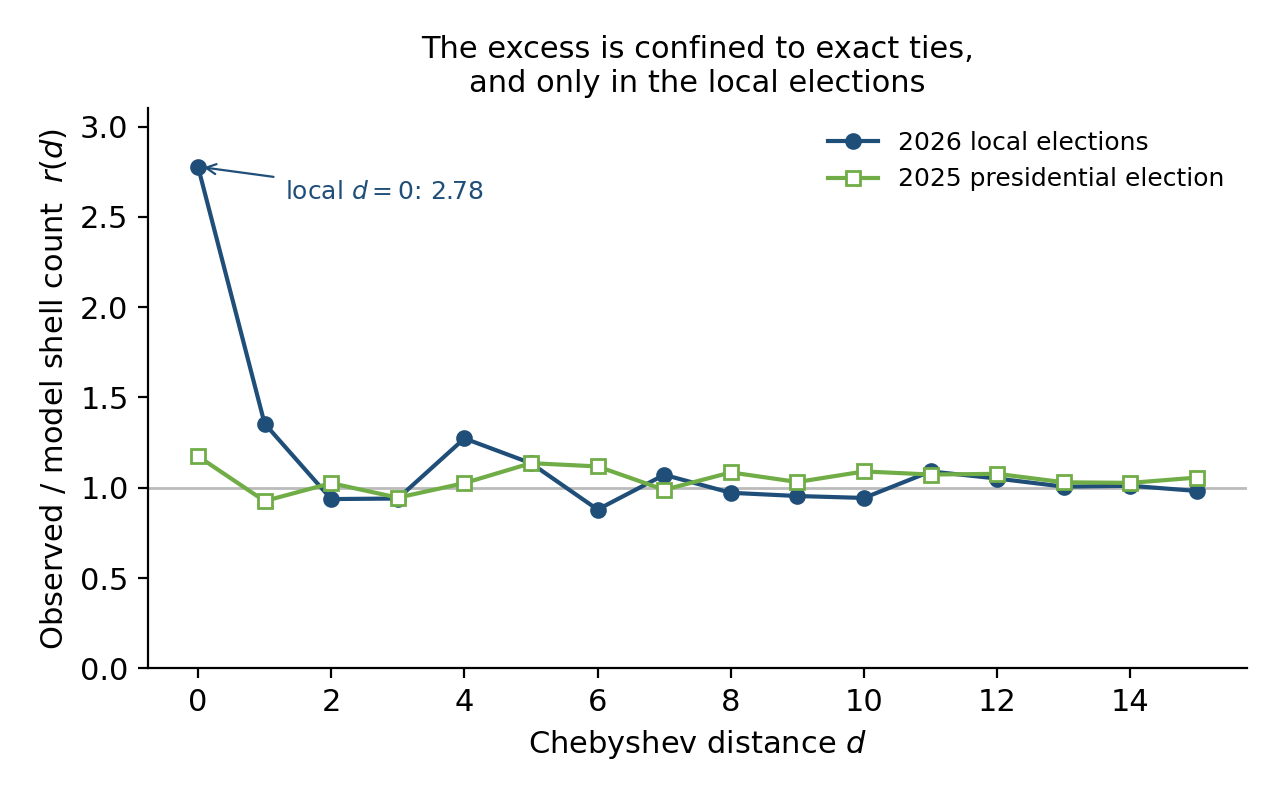
\includegraphics[keepaspectratio,alt={Figure 2}]{figs/fig2_ratio.png}}
\caption{Figure 2}
\end{figure}

\textbf{Figure 2.} Shell ratio \(r(d)\) for the two elections. The
presidential election (green) is consistent with 1 everywhere including
\(d = 0\); the local elections (blue) depart only at \(d = 0\) (2.78).

The ratio \(r(d)\) is flat at 0.93--1.17 across the entire range
including \(d = 0\). The type composition (model expectation: day·day
2.78, early·early 2.35, mixed 0.86; observed: 6, 0, 1) is consistent
with the model (\(P(\text{zero early of 7} \mid 39\%) \approx 3\%\)).
The pre-specified prediction --- \textasciitilde17 twins under a
structural mechanism --- is decisively rejected
(\(P(\ge 17 \mid 6.0) \approx 10^{-4}\)).

The reversal of type composition between the elections (early 6/9
\(\to\) early 0/7) follows naturally from the packing-density principle:
twins track not a particular vote type but \emph{wherever counts bunch
up small}. In Jeonnam's local race the landslide (B's share 8\%)
compressed the early-voting B-axis to 42--57 votes; in the presidential
race the election-day units of rural Honam played that role. This
refutes the popular notion of an early-voting-specific anomaly with data
--- while reaffirming that the localization of §4.3 (why the
\emph{least}-expected type?) cannot be explained by any property of
elections in general.

\subsection{6. Re-evaluating the public
analysis}\label{re-evaluating-the-public-analysis}

The public analysis {[}8{]} that sparked the debate used the
decomposition (number of pairs) × (similar-pair rate) × (tie probability
\textbar{} similar). This skeleton is a hand-computed version of our
sideband estimator and is structurally sound. The problem is the
provenance of its parameters.

\textbf{Incheon.} The coin-model tie probability 0.903\% (which we
re-verify) and the birthday-problem pair count are correct, but
``suppose about 1\% of pairs are similar'' is an assumption. Measured
(by inverting the same decomposition against our shell counts), the
actual similar-pair rate is \textbf{0.012\% --- about 82× smaller}. The
158 early-voting units of Incheon contain just two near pairs at
\(d \le 10\). The expected number of twins is therefore not the claimed
0.84 but 0.0137 (canonical) = 0.0146 (sideband), and
\(P(\ge 1) = 1.4\%\). By count magnitude (3,030/1,440), the Songdo twin
is single-handedly the rarest twin in the country. In fairness, Songdo
1- and 2-dong are de facto parameter twins (4,546 vs.~4,539 ballots;
homogeneous new-town districts), the one case where the
demographic-similarity story is visibly plausible --- favoring the
original analysis on the \emph{conditional} factor.

\textbf{The follow-up addendum.} The objection that assuming
\(p_1 = p_2\) inflates the tie probability is valid --- it is the mirror
image of our Proposition 1. However, the public code verification
offered in response draws a single \(p\) \textbf{shared by both units}
(\(X_1, X_2 \sim \mathrm{Bin}(n, p)\) with one Beta draw), thereby
re-assuming \(p_1 = p_2\); its agreement with the original number
(0.901\% vs.~0.906\%) is circular. Implemented as intended --- each unit
drawing \(p\) independently from its posterior --- the variance triples
and the tie probability becomes 0.524\% (a \(\sqrt{3}\) reduction).
Either way the order of magnitude stands, so ``the conclusion is roughly
unchanged'' holds in the narrow sense for the conditional factor. But
the tie probability is extremely sensitive to the \emph{true} difference
in support: 0.54\% at Δp = 1 pp, 0.11\% at 2 pp, 0.008\% at 3 pp,
\(\approx 0\) at 5 pp.~The effective definition of ``similar'' is thus
``true support within ±1.5 pp \emph{and} nearly equal size'' --- and the
measured fraction of such pairs is 0.012\%. The thread polished the
approximately-correct conditional factor while leaving the 80×-wrong
unconditional factor untouched.

\textbf{Gwangju--Jeonnam.} The original analysis's qualitative
directions --- tie probability grows as \(n\) falls and \(p \to 1\);
pairs grow as \(k^2\) --- are all correct, and indeed explain why the
Gwangju--Jeonnam expectation (1.47) is \textasciitilde100× Incheon's
(0.014). But no quantitative computation was performed before declaring
the result ``a naturally understandable coincidence.'' The measured
significance is 1.0--2.8\%: neither ``entirely natural'' (which would
imply tens of percent) nor ``an impossible coincidence'' is supported.

\subsection{7. Discussion}\label{discussion}

\subsubsection{7.1 Interpretation}\label{interpretation}

Three facts are established. (i) Twins are a base-rate phenomenon ---
the presidential election's seven twins match the model exactly. (ii)
The nine twins of the 2026 local elections are a \textasciitilde1\% tail
event relative to that base rate, a number stable across the entire
methodological spectrum (conditional / unconditional / model-free).
(iii) The excess is an atom at exact equality, localized four-fold.

What may be inferred? A frequentist 1\% is not a posterior probability
of fraud. The fraud hypothesis does not particularly predict this
pattern --- exact ties of tens of votes in districts decided by 60-point
margins --- so the likelihood ratio is near 1, and with a low prior and
no independent evidence the posterior barely moves. Meanwhile the public
scrutinizes dozens of statistics per election (selection effects
{[}5{]}), so the effective surprise of a face-value 1\% is smaller
still. In the opposite direction, the rhetoric of ``entirely natural''
is, as a sampling claim, off by a factor of \textasciitilde40 (§6). The
sentence the data licenses is exactly this: \textbf{it is rare
(\textasciitilde1\%), and rarity is not evidence of manipulation.}

Two hypotheses remain for the residual atom: a post-hoc-selected
coincidence, or a non-statistical cause confined to the 2026 local
elections' early voting (including reporting-pipeline artifacts upstream
of publication). The latter is discriminable by non-statistical means
(§7.3) --- a narrowing of the search space which is the product, not the
failure, of the statistical analysis.

\subsubsection{7.2 Limitations}\label{limitations}

\begin{enumerate}
\def\labelenumi{(\arabic{enumi})}
\tightlist
\item
  The fundamental limitation of post-hoc analysis of a single election:
  the hypothesis (the twin statistic itself) originated from the data.
  The presidential replication mitigates this by pre-specification, but
  a cause unique to the local elections survives it. (2) Each
  neighborhood is observed once, so within-neighborhood dispersion
  (\(\varphi\)) is unidentifiable. (3) The type localization (§4.3) is
  post hoc and its significance is reported at face value, before
  exploration correction. (4) The integrity verification (§2.4) excludes
  collection and transcription artifacts on our side, but errors
  upstream of official publication cannot be checked by re-reading the
  publication --- that is the domain of physical recounts. (5) A
  replication on the previous local elections (2022) remains undone; it
  would discriminate ``local elections in general'' from ``2026 only''
  and would sharpen, though not redirect, our conclusions.
\end{enumerate}

\subsubsection{7.3 Future work}\label{future-work}

\begin{enumerate}
\def\labelenumi{(\alph{enumi})}
\tightlist
\item
  The 2022 local elections under the identical pipeline; (b) extension
  to National Assembly elections (constituency level); (c)
  generalization of the sideband estimator --- arbitrary-dimension
  multivariate exact ties, shell weighting under heterogeneous noise
  scales.
\end{enumerate}

\subsection{8. Conclusion}\label{conclusion}

The nine twin counting units of the 2026 Korean local elections
constitute a tail event of roughly 1\% under any smooth stochastic model
(nationwide 0.64--0.94\%; Gwangju--Jeonnam 1.0--2.8\%). The figure is
identical whether obtained from a generative model conditioned on
observed parameters, an unconditional distributional model, or a
sideband extrapolation using no generative assumptions at all; and the
excess did not recur in the 2025 presidential election. Exact ties are a
natural phenomenon present in every election; the 2026 excess lies
within the range of rare but possible coincidence; and the final
identity of its residue belongs to verification outside statistics ---
source audits and physical recounts. The error shared by both camps of
the public controversy was the same: not measuring what is measurable.

\begin{center}\rule{0.5\linewidth}{0.5pt}\end{center}

\subsection{References}\label{references}

{[}1{]} Beber, B. and Scacco, A. (2012). What the numbers say: A
digit-based test for election fraud. \emph{Political Analysis}, 20(2),
211--234.

{[}2{]} Mebane, W. R. (2008). Election forensics: The second-digit
Benford's law test and recent American presidential elections. In
\emph{Election Fraud: Detecting and Deterring Electoral Manipulation},
Brookings Institution Press.

{[}3{]} Klimek, P., Yegorov, Y., Hanel, R., and Thurner, S. (2012).
Statistical detection of systematic election irregularities.
\emph{PNAS}, 109(41), 16469--16473.

{[}4{]} Kobak, D., Shpilkin, S., and Pshenichnikov, M. S. (2016).
Integer percentages as electoral falsification fingerprints.
\emph{Annals of Applied Statistics}, 10(1), 54--73.

{[}5{]} Gelman, A. and Loken, E. (2014). The statistical crisis in
science. \emph{American Scientist}, 102(6), 460--465.

{[}6{]} Grimes, D. R. (2016). On the viability of conspiratorial
beliefs. \emph{PLOS ONE}, 11(1), e0147905.

{[}7{]} Littlewood, J. E. (1953). \emph{A Mathematician's Miscellany}.
Methuen, London.

{[}8{]} Huh, M.-H. (2026). ``Two dongs matching at 3,030 and 1,440
votes: can such agreement be coincidental?'' Public social-media post
and addendum, June 2026 (in Korean).

{[}9{]} National Election Commission of Korea. Election statistics
system, counting results. info.nec.go.kr (accessed June 2026).

{[}10{]} Public Data Portal of Korea. NEC presidential election counting
results (2025-06-03). data.go.kr.

\begin{center}\rule{0.5\linewidth}{0.5pt}\end{center}

\subsection{Appendix A.
Reproducibility}\label{appendix-a.-reproducibility}

All figures and numbers are reproduced by the public repository's
scripts: \texttt{twin\_model.py} (canonical model),
\texttt{analyze\_national.py} (local elections: national, shells,
sideband), \texttt{analyze\_president.py} (presidential),
\texttt{bias\_demo.py} (numerical verification of Proposition 1),
\texttt{type\_decompose.py} (type decomposition),
\texttt{abinitio\_sim.py} (unconditional variant),
\texttt{verify\_twins.py} (data integrity, §2.4),
\texttt{paper/make\_figs.py} (figures). Raw crawls and cleaned data are
included.

\subsection{Appendix B. Acknowledgements and AI
disclosure}\label{appendix-b.-acknowledgements-and-ai-disclosure}

Anthropic's Claude (Fable 5) was used for analysis-design discussion,
code authoring, and manuscript drafting. Responsibility for verification
of all analyses and for the final conclusions rests with the author.

\end{document}
